\documentclass{beamer}
\usetheme{default}
%\usetheme{pittsburgh}
\usecolortheme{albatross}

%###############################################################################
%#
%# Saját színek:
%#
\definecolor{todobgszin}{rgb}{0.64000,0.78000,0.22000}
\definecolor{todofrszin}{rgb}{0.00000,0.50000,0.00000}
\definecolor{background}{rgb}{0.00000,0.29412,0.49804}
%#
%###############################################################################

\setbeamercolor{normal text}{fg=white}
\setbeamertemplate{navigation symbols}{} % Navigációs ikonok off

\usepackage[T1]{fontenc}
\usepackage[utf8]{inputenc}
\usepackage[english,magyar]{babel}

\usepackage{hyperref}
\usepackage{color}
\usepackage{graphics}

%# Hogy lehessen blokkokat megjegyzéssé tenni:
\usepackage{verbatim}

\usebackgroundtemplate{

\includegraphics[width=\paperwidth, height=\paperheight]{figures/background.jpg}
}

% Néhány konstans deklarációja:
\newcommand{\vikszerzo}{Debreceni Csaba \\ \footnotesize \texttt{(H1HNR5, <debrecenics @ gmail>)} \vskip10pt \normalsize Nádudvari György \\ \footnotesize \texttt{(ULQP9P, <ulqp9p @ gmail>)} \normalsize}
\newcommand{\vikkonzulens}{Semeráth Oszkár és Szárnyas Gábor}
\newcommand{\vikcim}{Modellalapú szoftvertervezés \\ Házi feladat - 1. fázis}

%###############################################################################
%#
%# Footer definíció a szokásos címek beírásához.
%#
%# Csúnya hacket tartalmaz!!!
%# A "{footline}{#1}" utáni \textcolorral egy háttérszínnel megegyező "y"
%# karaktert írunk ki, hogy ne ugráljanak a dobozok a diákon.
%# Ha ez elmarad, akkor az alapvonal alá nyúló karaktereket (pl. g, y stb.)
%# tartalmazó stringek esetén eltérő magasságban lesz a footer, mint azoknál
%# amelyek csak az alapvonalra illeszkedő karaktereket tartalmaznak.
%#
\newcommand{\setfootline}[1]{\setbeamertemplate{footline}{\setbeamercolor{footline}{fg=white}\begin{beamercolorbox}[sep=1cm,wd=\textwidth,ht=1cm,left]{footline}{#1}\textcolor{background}{y}\end{beamercolorbox}}}
%#
%###############################################################################

%###############################################################################
%#
%# Saját eszközök:
%#
\newcommand{\todo}[1]{\fcolorbox{todofrszin}{todobgszin}{\emph{TODO: #1}}}
\newcommand{\angolul}[1]{\foreignlanguage{english}{#1}}
%#
%###############################################################################

\hypersetup{
    bookmarks=true,            % show bookmarks bar?
    unicode=true ,             % non-Latin characters in Acrobat’s bookmarks
    pdftitle={\vikcim},        % title
    pdfauthor={\vikszerzo},    % author
    pdfnewwindow=true,         % links in new window
    colorlinks=true,           % false: boxed links; true: colored links
    linkcolor=black,           % color of internal links
    citecolor=black,           % color of links to bibliography
    filecolor=black,           % color of file links
    urlcolor=black             % color of external links
}

%###############################################################################
%#
%#                     CÍM:
%#
\title{\vikcim}
\author{\vikszerzo \\ [0.5cm] \normalsize{Konzulensek: \vikkonzulens}}
\date{2013. március 20.}

%#
%###############################################################################

%###############################################################################
%#
%#                    DOKUMENTUMTÖRZS
%#
\begin{document}

%# Hogy ne kelljen a section-nek és a frametitle-nek is megadni ugyanazt a 
%# címet:
\newcommand{\slidecim}{}

%###############################################################################
%#
%#                    1. DIA:
%#
\section{Cím lap}
\begin{frame}[plain]
\titlepage
\end{frame}
%#
%###############################################################################

%###############################################################################
%#
%#                    A FELADAT
%#
\renewcommand{\slidecim}{A feladat}
\section{\slidecim}
\setfootline{Interstellar Overdrive}
\begin{frame}[t]
\frametitle{\slidecim}
\begin{itemize}
    \item Eredményjelző és egy automatikus jegyzőkönyv generátor
    \item Az 1. fáziban:
        \begin{itemize}
            \item Követelményanalízis
                \begin{itemize}
                     \item Magasszintű követelmények megfogalmazása az elkészítendő rendszerrel szemben
                     \item Mit kell/szeretnénk megvalósítani?
                     \item Kimenet: Use case diagram
                \end{itemize}
            \item Domain modellezés
                \begin{itemize}
                     \item Magasszintű domain modell elkészítése
                     \item Mik a domain elemei?
                     \item Kimenet: EMF modell és OCL kényszerek
                \end{itemize}
            \item Dinamikus modellezés
                \begin{itemize}
                    \item A kijelző működésének leírása
                    \item Milyen állapotai vannak a rendszerünknek?
                    \item Kimenet: Yakindu state chartok
                \end{itemize}
        \end{itemize}         
\end{itemize}
\end{frame}
%#
%###############################################################################

%###############################################################################
%#
%#                    USE CASE PÉLDA _ PIROSLAPOK KEZELÉSE
%#
\renewcommand{\slidecim}{Use case részlet - Piros lapok kezelése}
\section{\slidecim}
\setfootline{Green Is the Colour}
\begin{frame}[c]
\frametitle{\slidecim}
\begin{figure}[!ht]
\centering
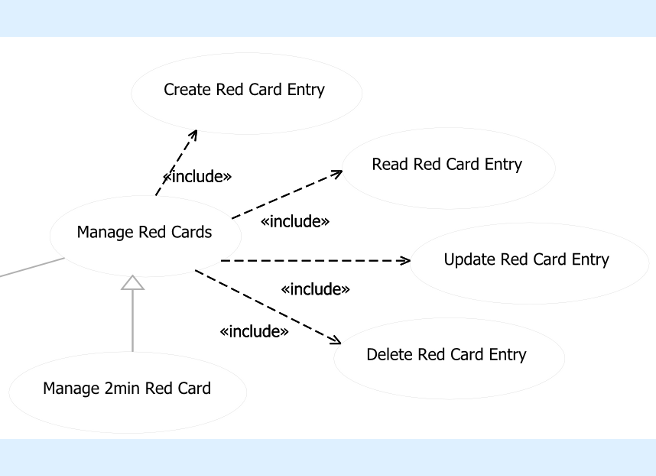
\includegraphics[width=100mm, keepaspectratio]{figures/use_case_red_cards.png}
\end{figure}
\end{frame}
%#
%###############################################################################

%###############################################################################
%#
%#                    DOMAIN MODELL 1
%#
\renewcommand{\slidecim}{Domain modell}
\section{\slidecim}
\setfootline{Wearing the Inside Out}
\begin{frame}[c]
\frametitle{\slidecim}
\begin{figure}[!ht]
\centering
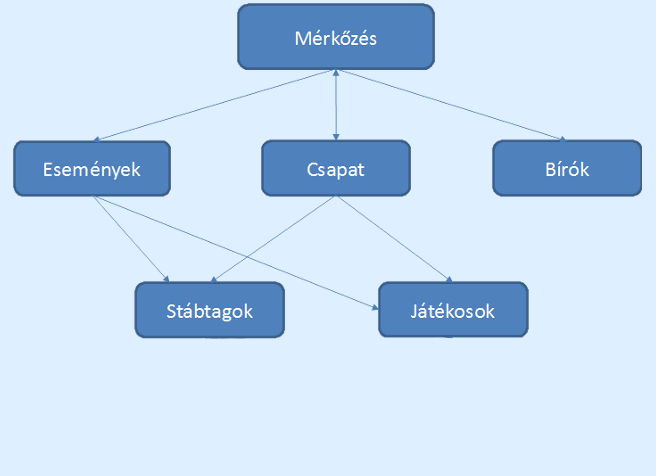
\includegraphics[width=100mm, keepaspectratio]{figures/domain_modell_001.png}
\end{figure}
\end{frame}
%#
%###############################################################################

%###############################################################################
%#
%#                    DOMAIN MODELL 2
%#
\renewcommand{\slidecim}{Domain modell}
\section{\slidecim}
\setfootline{Wearing the Inside Out}
\begin{frame}[c]
\frametitle{\slidecim}
\begin{figure}[!ht]
\centering
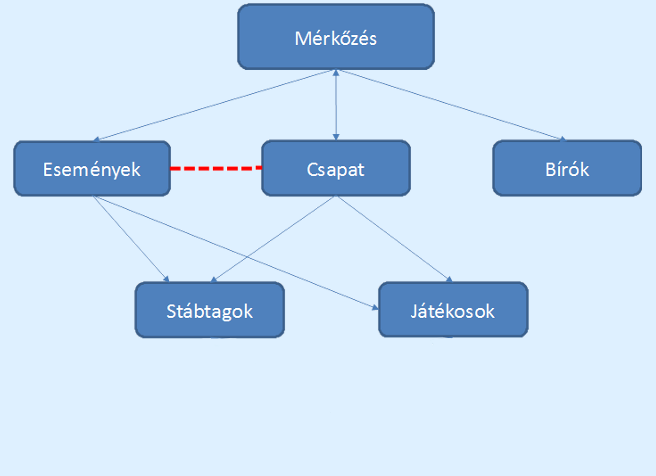
\includegraphics[width=100mm, keepaspectratio]{figures/domain_modell_002.png}
\end{figure}
\end{frame}
%#
%###############################################################################

%###############################################################################
%#
%#                    DOMAIN MODELL 3
%#
\renewcommand{\slidecim}{Domain modell}
\section{\slidecim}
\setfootline{Wearing the Inside Out}
\begin{frame}[c]
\frametitle{\slidecim}
\begin{figure}[!ht]
\centering
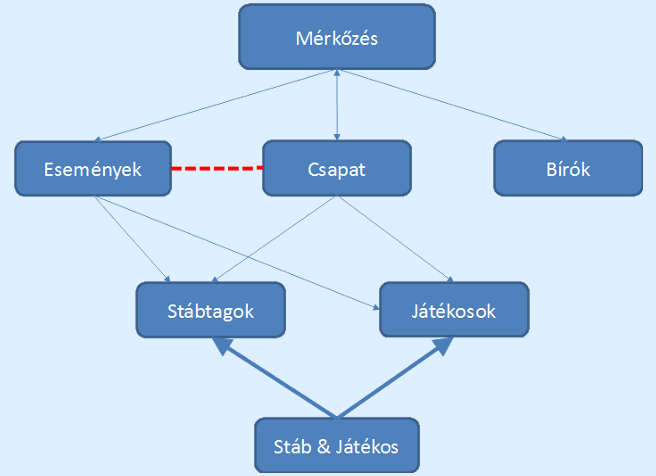
\includegraphics[width=100mm, keepaspectratio]{figures/domain_modell_003.png}
\end{figure}
\end{frame}
%#
%###############################################################################

%###############################################################################
%#
%#                    OCL KÉNYSZEREK
%#
\renewcommand{\slidecim}{OCL kényszerek}
\section{\slidecim}
\setfootline{Don't Leave Me Now}
\begin{frame}[c]
\frametitle{\slidecim}
\begin{itemize}
    \item Modell alapú kényszerek
    \begin{itemize}
        \item A modell megalkotásakor nem tudtunk őket kikényszeríteni
    \end{itemize}
    \item Szabály alapú kényszerek
    \begin{itemize}
        \item A játék speciális szabályaiból adódnak
    \end{itemize}
    \item Derived features
    \begin{itemize}
        \item Ezeket a feature-ket is meg lehet/kell fogalmazni OCL kényszerkén
    \end{itemize}
\end{itemize}
\end{frame}
%#
%###############################################################################

%###############################################################################
%#
%#                    ÁLLAPOT DIAGRAM - IDŐ MEGVALÓSÍTÁSA
%#
\renewcommand{\slidecim}{Állapot diagram - Idő megvalósítása}
\section{\slidecim}
\setfootline{Time}
\begin{frame}[c]
\frametitle{\slidecim}
\begin{figure}[!ht]
\centering
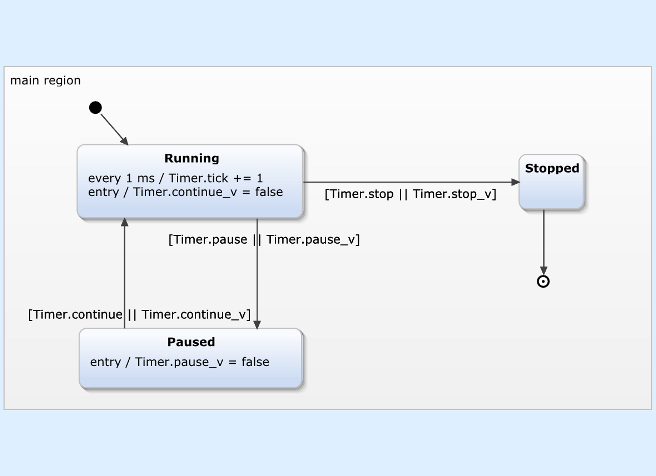
\includegraphics[width=100mm, keepaspectratio]{figures/state_chart_main_region.png}
\end{figure}
\end{frame}
%#
%###############################################################################

%###############################################################################
%#
%#                    EXTRÁK
%#
\renewcommand{\slidecim}{Extrák}
\section{\slidecim}
\setfootline{When You're In}
\begin{frame}[c]
\frametitle{\slidecim}
\begin{itemize}
    \item Szabályrendszerben
    \begin{itemize}
        \item Plusz attribútumok a mérkőzéshez
        \item Büntetők kupameccs esetén
        \item 2 perces visszaszámlálás
    \end{itemize}
    \item Technológiában
    \begin{itemize}
        \item Derived feature-k Incquery-vel megvalósítva
    \end{itemize}
\end{itemize}
\end{frame}
%#
%###############################################################################

%###############################################################################
%#
%#                    PROBLÉMÁK, KIHÍVÁSOK
%#
\renewcommand{\slidecim}{Problémák, kihívások}
\section{\slidecim}
\setfootline{Eclipse}
\begin{frame}[c]
\frametitle{\slidecim}
\begin{itemize}
\item Amivel nem volt gond:
    \begin{itemize}
        \item A domain ismeretével
    \end{itemize}
\item Amivel viszont igen:
    \begin{itemize}
        \item A domain ismeret eltérő szintje a csapatagoknál
        \item Eszközök együttműködése
            \begin{itemize}
                \item Papyrus vs. Yakindu
            \end{itemize}             
        \item Yakinduban események küldés (raise)
             \begin{itemize}
                \item Események helyett/mellett boolean változókat kell használni
             \end{itemize}
        \item Az egyes tervezési lépések közötti határok megtalálása
            \begin{itemize}
                \item Mi a domain modell része?
                \item Mi kerül egy állapot diagramra?
                \item Hogy lesz ebből egész?
            \end{itemize}             
    \end{itemize}
\end{itemize}
\end{frame}
%#
%###############################################################################

%###############################################################################
%#
%#                    ÖSSZEFOGLALÁS - ELÉRT EREDMÉNYEK
%#
\renewcommand{\slidecim}{Összefoglalás - Elért eredmények}
\section{\slidecim}
\setfootline{High Hopes}
\begin{frame}[c]
\frametitle{\slidecim}
\begin{itemize}
\item Elkészült:
    \begin{itemize}
        \item A rendszer funkcióinak use case diagramja
        \item A domain modell EMF-ben
        \item OCL kényszerek
        \item Állapot diagram a rendszer működéséről
    \end{itemize}
\end{itemize}
\end{frame}
%#
%###############################################################################

%###############################################################################
%#
%#                    KÉRDÉSEK
%#
\section{Kérdések?}
\setfootline{\angolul{Is There Anybody Out There?}}
\begin{frame}[c]
\frametitle{}
\begin{center}
\huge{\textbf{Kérdések?}}\\
\begin{figure}[!ht]
\centering

\includegraphics[width=20mm, keepaspectratio]{figures/questions.png}
\end{figure}
\end{center}
\end{frame}
%#
%###############################################################################

%###############################################################################
%#
%#                    THE END
%#
\section{Vége}
\setfootline{\angolul{Comfortably Numb}}
\begin{frame}[c]
\frametitle{}
\begin{center}
\huge{\textbf{Köszönjük a figyelmet!}}
\end{center}
\end{frame}
%#
%###############################################################################

%###############################################################################
%#
%#                    SABLON DIA
%#
\begin{comment}

\renewcommand{\slidecim}{•}
\section{\slidecim}
\setfootline{\todo{Keep floyding}}
\begin{frame}[c]
\frametitle{\slidecim}
\todo{•}
\end{frame}

\end{comment}
%#
%###############################################################################

\end{document}
